\chapter{Implementatie}
In het vorige hoofdstuk is uitgelegd wat de methode is voor het testen, maar hoe vertalen deze vereisten naar een werkende test programma? In dit hoofdstuk zal deze vertaling uitgelegd worden die op deze thesis is toegepast. 

Vooraleer met de eigenlijke uitwerking kon gebeuren, wordt eerst uitgelegd welke systemen gekozen zijn en waarom. 
Vervolgens zullen de gekozen systemen in meer detail besproken worden, waarna de uitwerking van de testsoftware aanbod komt. Tenslotte zullen de verschillende stappen van de testprocedure overlopen worden met hun gedetailleerde parameters.  
\section{Selectie van de DBMS's}
Voor de selectie van de systemen is er onderzocht of een systeem een bepaalde eigenschap al dan niet ondersteunt. In het totaal zijn er 5 verschillende eigenschappen waarop de selectie is gebaseerd. 

\paragraph{Vrije software} Om testen tussen verschillende DBMS's te kunnen vergelijken op een gelijkaardige infrastructuur, is het nodig dat deze software kan geïnstalleerd worden op de eigen infrastructuur, een extra selectie criteria is dat de systemen gratis aangeboden worden. 

\paragraph{Persistentie} Voor het testen van de beschikbaarheid van de data, is het een voordeel dat de data op harde schijf aanwezig is: bij een herstel dient er minder data over het netwerk gestuurd te worden. Om deze reden hebben persistente systemen een voorkeur op deze die de data enkel in geheugen houden. 

\paragraph{Replicatie} Eén van de testen is de beschikbaarheidstest, indien de data maar op een enkele server opgeslagen is, zal de data op de uitgeschakelde server niet langer beschikbaar zijn. Met replicatie zal de data op verschillende servers opgeslagen worden en zal de data in theorie nog beschikbaar zijn in het geval van een enkele uitgeschakelde server. 

\paragraph{Data distributie} Het is de bedoeling om systemen te testen die een grote hoeveelheid data kunnen opslaan. Om aan deze vereiste te voldoen, is het nodig dat elke server niet al de data opslaat bij een grote dataset. Hiervoor zijn er wel voldoende aantal servers nodig, bij te weinig servers is elke server nodig om aan de replicatie vereiste te voldoen. 

\paragraph{Ondersteuning voor verschillende query methodes} Bij de testen worden er 5 soorten queries uitgevoerd: invoegen, aanpassen, verwijderen en het opvragen van een individueel of meerdere record. De DBMS moet ondersteuning voor deze queries. De eerste 4 kunnen in al de systemen geïmplementeerd worden met één of meerdere queries. Maar het opvragen van meerdere queries, een scan query, is in bepaalde systemen niet ondersteund. Deze scan query is een query waar het record met een bepaalde sleutel wordt opgevraagd en een aantal records dat hierop volgt, het is \textit{geen} query met een begin en eind sleutel. 

Voor alle systemen besproken in sectie \ref{sec:BesprekingDBMS}, is het eerste criterium voldaan. De overige 4 criteria zijn samengevat in tabel \ref{table:vergelijkingNosql}.

Een korte verklaring bij enkele van de waarden uit de tabel. Bij \textit{Redis} is er sprake van een snapshot of een log voor de persistentie, de eigenlijke database wordt enkel in het geheugen gehouden. Hierdoor is er maar half sprake , hierdoor kan de database herstelt worden maar is deze niet in het geheugen. \\
Bij \textit{replicatie} zijn er 2 mogelijke configuraties: master-slave waarbij er verschillende instanties verschillende functies hebben en één de baas is, of master-master waarbij ze allemaal gelijk zijn. \\
Bij \textit{aanpassen} zijn er systemen die voor een update al de verschillende kolom waarden nodig hebben of maar 1 kolom per waarde ondersteunen. \\
Bij \textit{scan} is er bij enkele systemen enkel ondersteuning voor het lezen tussen 2 verschillende sleutels. Met het iteratief opvragen van elementen tussen 2 sleutels en het lezen van een beperkte hoeveelheid data, is het mogelijk om een scan query uit te voeren, maar dit is maar halve ondersteuning. 

Bij de selectie is er naast de 4 criteria, ook gekozen voor systemen van verschillende datamodellen. Samen met mijn collega Arnaud Schoonjans \cite{thesisArnaud}, zijn er in 7 verschillende systemen verder onderzocht. In deze thesis zijn  HBase, MongoDB en Pgpool-II verder onderzocht, in de thesis van mijn collega zijn dit Cassandra, Apache CouchDB, Riak en MySQL.  
 
% Table generated by Excel2LaTeX from sheet 'Sheet1'
\begin{table}[htbp]
  \centering
  \resizebox{\columnwidth}{!}{%
    \begin{tabular}{ll|lllll}
          &       & \multirow{2}[1]{*}{Persistentie} & \multirow{2}[1]{*}{Replicatie} & \multirow{2}[1]{*}{Datadistributie} & \multicolumn{2}{c}{Query soort} \\
    
          &       &       &       &       & Aanpassen & Scan \\ \hline
    \multirow{2}[1]{*}{Column} & Cassandra & Ja    & Master-Master & Ja    & Ja    & Half \\
          & HBase & Ja    & Master-Slave & Ja    & Ja    & Ja \\
          
          \hline
    \multirow{3}[0]{*}{Document} & Apache  & \multicolumn{1}{l}{\multirow{2}[0]{*}{Ja}} & \multicolumn{1}{l}{\multirow{2}[0]{*}{Master-Master}} & \multicolumn{1}{l}{\multirow{2}[0]{*}{Ja}} & \multicolumn{1}{l}{\multirow{2}[0]{*}{Nee}} & \multicolumn{1}{l}{\multirow{2}[0]{*}{Ja}} \\
          & CoucheDB & \multicolumn{1}{l}{} & \multicolumn{1}{l}{} & \multicolumn{1}{l}{} & \multicolumn{1}{l}{} & \multicolumn{1}{l}{} \\
          & MongoDB & Ja    & Master-Slave & Ja    & Ja    & Ja \\
          
          \hline
    \multirow{6}[0]{*}{Key-Value} & LightCloud & \multicolumn{1}{l}{\multirow{2}[0]{*}{Ja}} & \multicolumn{1}{l}{\multirow{2}[0]{*}{Master-Master}} & \multicolumn{1}{l}{\multirow{2}[0]{*}{Ja}} & \multicolumn{1}{l}{\multirow{2}[0]{*}{Nee}} & \multicolumn{1}{l}{\multirow{2}[0]{*}{Ja}} \\
          & (Tokyo) & \multicolumn{1}{l}{} & \multicolumn{1}{l}{} & \multicolumn{1}{l}{} & \multicolumn{1}{l}{} & \multicolumn{1}{l}{} \\
          & MemcacheDB & Ja    & Master-Slave    & Nee   & Nee   & Ja \\
          & Redis & Half & Master-Slave & Nee  & Ja    & Half \\
          & Riak  & Ja    & Master-Master & Ja    & Nee   & Half \\
          & Voldemort & Ja    & Master-Master & Ja    & Nee   & Nee \\
          
          \hline
    \multirow{3}[0]{*}{Relationeel} & MySQL & Ja    & Master-Slave & Nee   & Ja    & Ja \\
    	  & PostgreSQL & Ja    & Master-Slave & Nee   & Ja    & Ja \\
          & Pgpool-II & \multicolumn{1}{l}{\multirow{2}[0]{*}{Ja}} & \multicolumn{1}{l}{\multirow{2}[0]{*}{Master-Slave}} & \multicolumn{1}{l}{\multirow{2}[0]{*}{Ja}} & \multicolumn{1}{l}{\multirow{2}[0]{*}{Ja}} & \multicolumn{1}{l}{\multirow{2}[0]{*}{Ja}} \\
          & (PostgreSQL) & \multicolumn{1}{l}{} & \multicolumn{1}{l}{} & \multicolumn{1}{l}{} & \multicolumn{1}{l}{} & \multicolumn{1}{l}{} \\
    \end{tabular}%
    }
    \caption{Ondersteuning van de besproken DBMS's naar de selectie criteria. }
  \label{table:vergelijkingNosql}%
\end{table}%

\section{Gedetailleerde bespreking van de geselecteerde DBMS's}
In dit gedeelte zal elk geselecteerd systemen in meer detail uitgelegd worden. Een gemeenschappelijk element bij al deze systemen is dat niet alle instanties dezelfde functie hebben, in andere DBMS's hebben alle instanties dezelfde functie bij het wat de installatie en configuratie kan vereenvoudigen. 

Voor elk van de geselecteerde systemen zal de aangeboden API besproken worden met een blik op de datastructuur, daarna zal de systeem architectuur besproken worden. 

\subsection{HBase}

\subsubsection{Data structuur\cite{george2011hbase}}
De data in HBase is gestructureerd in tabellen, bij het aanmaken wordt er een schema voor de tabel gemaakt. Voor elke tabel kunnen de verschillende kolommen meegegeven worden samen met een \textit{kolom familie} voor elke kolom, maar de kolommen kunnen ook gespecificeerd worden bij het schrijven van data. De gegevens per \textit{kolom familie} hebben dezelfde prefix en zullen fysisch samen opgeslagen worden. Indien verschillende kolommen tegelijk worden gelezen of geschreven, is het aangeraden om deze dezelfde \textit{kolom familie} te geven. 

De operaties beschikbaar in dit systeem zijn: get (verkrijgen), put (invoegen), scan en delete (verwijderen). Het aanpassen van gegevens wordt uitgevoerd via een put waarbij een enkele kolom waarde van een record kan aanpast worden. Een scan operatie heeft geen optie om het aantal op te halen records te bepalen maar er kan wel bepaald worden in welke batch grootte (bytes) de records opgehaald moeten worden. Doordat er geweten is hoe groot een individueel record is én hoeveel records er opgevraagd worden, kan de cache grootte zo bepaald worden dat er maar een enkele datacommunicatie nodig is. 

\subsubsection{Architectuur\cite{george2011hbase}}
De gedistribueerde versie van HBase is afhankelijk van 2 andere software systemen, namelijk Zookeeper\cite{hunt2010zookeeper} en Hadoop\cite{borthakur2007hadoop}, en volgt hiermee de structuur van Google's BigTable\cite{chang2008bigtable} die op zijn beurt afhankelijk is van Chubby\cite{burrows2006chubby} en Google File System\cite{ghemawat2003google}. Een overzicht van de architectuur bevindt zich in figuur \ref{fig:Hbase-structure}. De 3 systemen van HBase zullen kort besproken worden, van HBase naar Zookeeper en Hadoop. 

\begin{figure}[ht!]
\centering
\includegraphics[width=\linewidth]{img/Hbase-structure.png}
\caption{Volledige systeemarchitectuur van HBase met Hadoop en Zookeeper. Bron \cite{ChinHBaseComprehensive}}
\label{fig:Hbase-structure}
\end{figure}

\paragraph{HBase\cite{george2011hbase}} HBase is een master/slave systeem welke bestaat uit een HMaster en een HRegionServer. De \textit{HMaster} is verbonden met Zookeeper en houdt op deze manier de status van de HRegionServers in het oog. Daarnaast is deze ook verantwoordelijk voor het toewijzen van data verantwoordelijkheden, zoals het opsplitsen een tabel over verschillende regio's indien een tabel groeit en het toewijzen van een regio aan een HRegionServer.\\
De andere soort, een \textit{HRegionServer}, is verantwoordelijke voor de data in een of meerdere regio's en voor het beheren van deze regio's. Een regio is een deel van een tabel met daar in de feitelijke data die opgeslagen is in verschillende datanodes. Een HRegionServer zal consistentie en atomaire queries afdwingen in HBase op een enkele record.  

\paragraph{Hadoop\cite{borthakur2007hadoop}} HBase maakt gebruik van het Hadoop Distributed File System (HDFS), een gedistribueerd file systeem ontworpen om te werken op commodity hardware met een hoge fout tolerantie. HDFS heeft een master/slave architectuur en bestaat uit een enkele \textit{namenode}, de master server, die de naamruimte en toegangscontrole onderhoudt, en \textit{datanode}s. De data wordt opgedeeld in blokken die door een verzameling van datanodes wordt opgeslagen, op deze manier is er data distributie. Deze master/slave configuratie zijn verschillende soorten van services en dient door de gebruiker zelf geconfigureerd te worden. \\
In de deze configuratie van HBase, is HDFS de methode om data persistent op te slaan met automatische replicatie en data distributie. Er is ook ondersteuning om de opslag naar Amazon S3 te doen in een gedistribueerde omgeving of deze op de lokale harde schrijf op te slaan bij een configuratie met slechts 1 server.\cite{george2011hbase}

\paragraph{Zookeeper\cite{hunt2010zookeeper}} Zookeeper is een service voor het coördineren van gedistribueerde applicatie processen, deze service biedt primitieven aan om synchronisatie, configuratieonderhoud en benaming te doen. Zookeeper is op zijn beurt een gedistribueerd master/slave systeem dat ontworpen is om snel te zijn bij dominantie van leesoperaties.  \\
HBase gebruikt Zookeeper onder andere voor het bijhouden van de status van regio server, hun locatie en hun verantwoordelijkheden. Dit verloopt met het toekennen van sessie die een een HRegionServer bijvoorbeeld de verantwoordelijkheid voor een Region geeft voor de volgende minuut. Tijdens deze periode kan geen enkele andere HRegionServer een bewerking doen op deze Region, uitgezonderd met de toestemming van de verantwoordelijke server. \cite{george2011hbase} Deze sessie duur kan geconfigureerd worden in Zookeeper met wordt in dit geval op de standaard 180 seconden gelaten. 

Dit is de globale structuur van het HBase systeem, in het totaal zijn er 5 verschillende soorten services: 2 voor Hadoop, 1 voor Zookeeper en 2 bij HBase. Enkele van deze services worden best gegroepeerd op een enkele instantie: de HDBS namenode, een Zookeeper instantie en de HMaster worden samen op een enkele instantie geplaatst, hetzelfde geldt voor een datanode en een HRegionServer. Zeker deze laatste heeft een extra performantie invloed: HBase detecteert dat er lokale opslag van de data is en de regio zal steeds deze lokale opslag hebben. Dit zorgt bij leesacties voor een performantie verbetering aangezien de data lokaal gelezen kan worden.

De configuratie van de verschillende systemen gebeurt door middel van configuratiebestanden voor elke service waarna de verschillende systemen zich bij elkaar aanmelden en de volledige configuratie van Region's door het systeem zelf wordt gedaan.  

\subsection{MongoDB\cite{mongodb-manual}}

\subsubsection{Datastructuur}
De data in MongoDB is opgeslagen in een database, die op zijn beurt een collectie bevat. Het is niet nodig om een een database en collectie op voorhand aan te maken, deze worden automatisch aangemaakt bij het wegschrijven van data indien de collectie nog niet bestaat. Een record is in MongoDB een document en elk record kan verschillende velden hebben. Er zijn uitgebreide query mogelijkheden om data in te voegen, aan te passen, te verwijderen of een scan uit te voeren. Er is ook ondersteuning voor MapReduce\cite{dean2008mapreduce}. 

Bij het schrijven van data, kunnen verschillende eisen gesteld worden voor het voltooien van de actie, startende met de actie is over het netwerk verstuurd, de primary heeft de data geschreven tot een meerderheid van de secondaries heeft de data weg geschreven. \\ Bij het lezen kan men kiezen om de data te lezen van de primary, secondary of de dichtstbijzijnde node. Afhankelijk van de gekozen acties, kan er verondersteld worden dat er een verschillende consistentie garantie zal zijn. Een overzicht van al de mogelijkheden, kan teruggevonden worden in tabel \ref{table:mongodb-query-opties}. Indien er in de tekst verder niet gespecificeerd wordt welke lees of schrijf query er wordt gebruikt zijn dit de standaard methodes, respectievelijk primary en normal. 

\begin{table}[ht!]
	\centering
	\begin{tabular}{l|l}
		\multicolumn{2}{c}{\textbf{Lees acties}} \\ 
		\textbf{Benaming} & \textbf{Omschrijving} \\ \hline
		Primary & Enkel lezen van de primary \\
		\multirow{2}[1]{*}{PrimaryPreferred} & Lezen van de primary, behalve als de primary  \\
		& onbeschikbaar is, lees dan van secondary. \\
		Secundary & Enkel lezen van een secondary \\
		\multirow{2}[1]{*}{SecundaryPreferred} & Lezen van een secondary, behalve als er geen secondary  \\
				& onbeschikbaar is, lees dan van de primary. \\
		\multirow{2}[1]{*}{Nearest} & Lees van de instantie met de laagste netwerk \\
				& vertraging, ongeachte het een primary of secondary is. \\
		\multicolumn{2}{c}{\textbf{}} \\ 		
		
		\multicolumn{2}{c}{\textbf{Schrijf acties}} \\ 
		\textbf{Benaming} & \textbf{Omschrijving} \\ \hline
		Normal & Wacht tot weggeschreven naar het netwerk socket. \\
		\multirow{1}[1]{*}{Safe} & Wacht op bevestiging van de primary    \\
		
		\multirow{2}[1]{*}{fsync$\_$safe} & Wacht op bevestiging van de primary tot  \\
				& de data is weggeschreven naar harde schijf.  \\
		\multirow{2}[1]{*}{Replica acknowledged} & Wacht op bevestiging van primary  \\
				& en één secondary. \\
		\multirow{1}[1]{*}{Majority} & Wacht op bevesting van meerderheid van de servers  \\
	\end{tabular}
	\caption{MongoDB: Mogelijke opties bij lees- en schrijfqueries}
	\label{table:mongodb-query-opties}
\end{table}

\subsubsection{Architectuur}
MongoDB is een DBMS dat de vereisten van replicatie en data distributie op een gelaagde manier tot uitvoering brengt. In eerste instantie zal deze de replicatie vereisten invullen, hierboven zal horizontale schaalbaarheid ondersteund worden. 

\begin{figure}[ht!] 
\centering
	\subfigure[Drie leden van een replica set met een primary en 2 secondaries. ]{\label{fig:mongodb-replicaset} 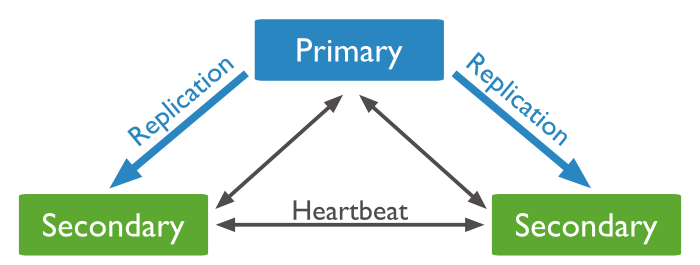
\includegraphics[width=0.40\textwidth]{img/mongodb-replica-set-primary-with-two-secondaries}}
	\hfill
	\subfigure[Een voorbeeld cluster voor productie met 2 mongos, 3 shards en 3 configuratie servers.]{\label{fig:mongodb-sharding} 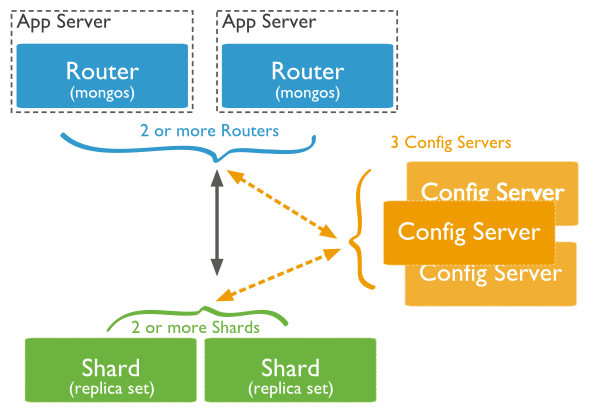
\includegraphics[width=0.50\textwidth]{img/mongo-sharded-cluster-production-architecture}}
	\caption{MongoDB Architectuur voor replicatie en datadistributie. Bron figuur link: \cite{mongodb-replicaset}, rechts: \cite{mongodb-shard}}
	\label{fig:mongodb-architectuur}
\end{figure}

\paragraph{Replicatie\cite{mongodb-replicaset}} Replicatie in MongoDB gebeurt door middel van een master/slave configuratie tussen verschillende \textit{MongoD} instanties, of in hun termen primary/secondaries. Deze instanties verkiezen zelf hun primary die verantwoordelijk is voor het afhandelen van de schrijfacties, de data zal vervolgens gerepliceerd worden naar de secondaries, of dit synchroon of asynchroon gebeurt is afhankelijk van de optie bij de schrijfactie. Een verzameling van deze MongoD instanties wordt een \textit{replicaset} genoemd. Het is slechts mogelijk om een instantie tot een enkele set toe te voegen. De data is beschikbaar zo lang er meer dan de helft van de servers beschikbaar zijn. 

\paragraph{Data distributie\cite{mongodb-shard}} Horizontale schaalbaarheid wordt in MongoDB bereikt door verschillende replicaset's of een enkele MongoD instantie te combineren tot een cluster. In het geval van de tweede keuze, zal de data niet gerepliceerd worden en wordt om deze reden niet aangeraden voor productie. 
\subparagraph{Shards} Sharding gebeurt automatisch op een collectie nadat is aangegeven dat men deze wilt verdelen over de gespecificeerde delen. Voor het uitvoeren van deze sharding zijn er nog 2 extra servers types nodig: configuratie servers en toegangsserver. 
\subparagraph{Configuratie servers} De configuratie servers slaan de meta data van de cluster op zoals de verschillende shards en replicaset's. Deze configuratie set bestaat uit 1 tot 3 servers, waarvoor naar productie 3 servers aangeraden is.
\subparagraph{Toegangsserver} De toegangsserver haalt de configuratie op uit de configuratie servers en biedt toegang voor de gebruiker aan tot de cluster. Er kunnen een onbepaald aantal toegangsservers zijn in cluster. 

De configuratie van de verschillende delen bestaat uit verschillende technieken. Bij replicatie krijgt elke set een naam die in de configuratiebestanden van elke configuratie wordt gezet, nadien wordt één instantie op de hoogte gebracht van de locatie van de andere instanties. Bij de cluster worden bij het opstarten van de toegangsservers de set van configuratieservers meegegeven, het opzetten van de verschillende shards gebeurt via een toegangsserver m.b.v. de API. 

\subsection{Pgpool-II (PostgreSQL)\cite{pgpool-doc}}
Pgpool-II kan op 4 verschillende manieren werken, in deze testen is er gekozen voor de replicatie mode omdat deze zowel replicatie, belastingsverdeling, failover en online recovery aanbiedt. Er is de mogelijkheid om ook data distributie aan te bieden maar dit is niet getest. Beide kunnen gecombineerd worden door de datadistributie voor de replicatie te zetten, hetzelfde principe als MongoDB. 

Datastructuur en de architectuur van Pgpool-II in replicatie mode komt nu in meer detail aanbod. 

\subsubsection{Datastructuur}
De data structuur en query mogelijkheden van Pgpool-II zijn gelijklopend aan deze van PostgreSQL. Net zoals in PostgreSQL bestaat het systeem uit een schema die verschillende databases kan bevatten. In een database zijn vervolgens verschillende tabellen die de records bevatten. Voor het opslaan van de data dient de volledige tabel met al de kolommen gespecificeerd zijn. 

Pgpool-II ondersteunt de volledige query mogelijkheden die in de testen nodig zijn. Er zijn enkele restricties ten opzichte van PostgreSQL die beschreven zijn op in de sectie \textit{Restrictions} van de documentatie\cite{pgpool-doc}. 

\subsubsection{Architectuur}
Een Pgpool-II infrastructuur bestaat uit 2 delen, een data en routing niveau, een overzicht is gegeven in figuur \ref{fig:Pgpool-structure}. 

\begin{figure}[ht!]
\centering
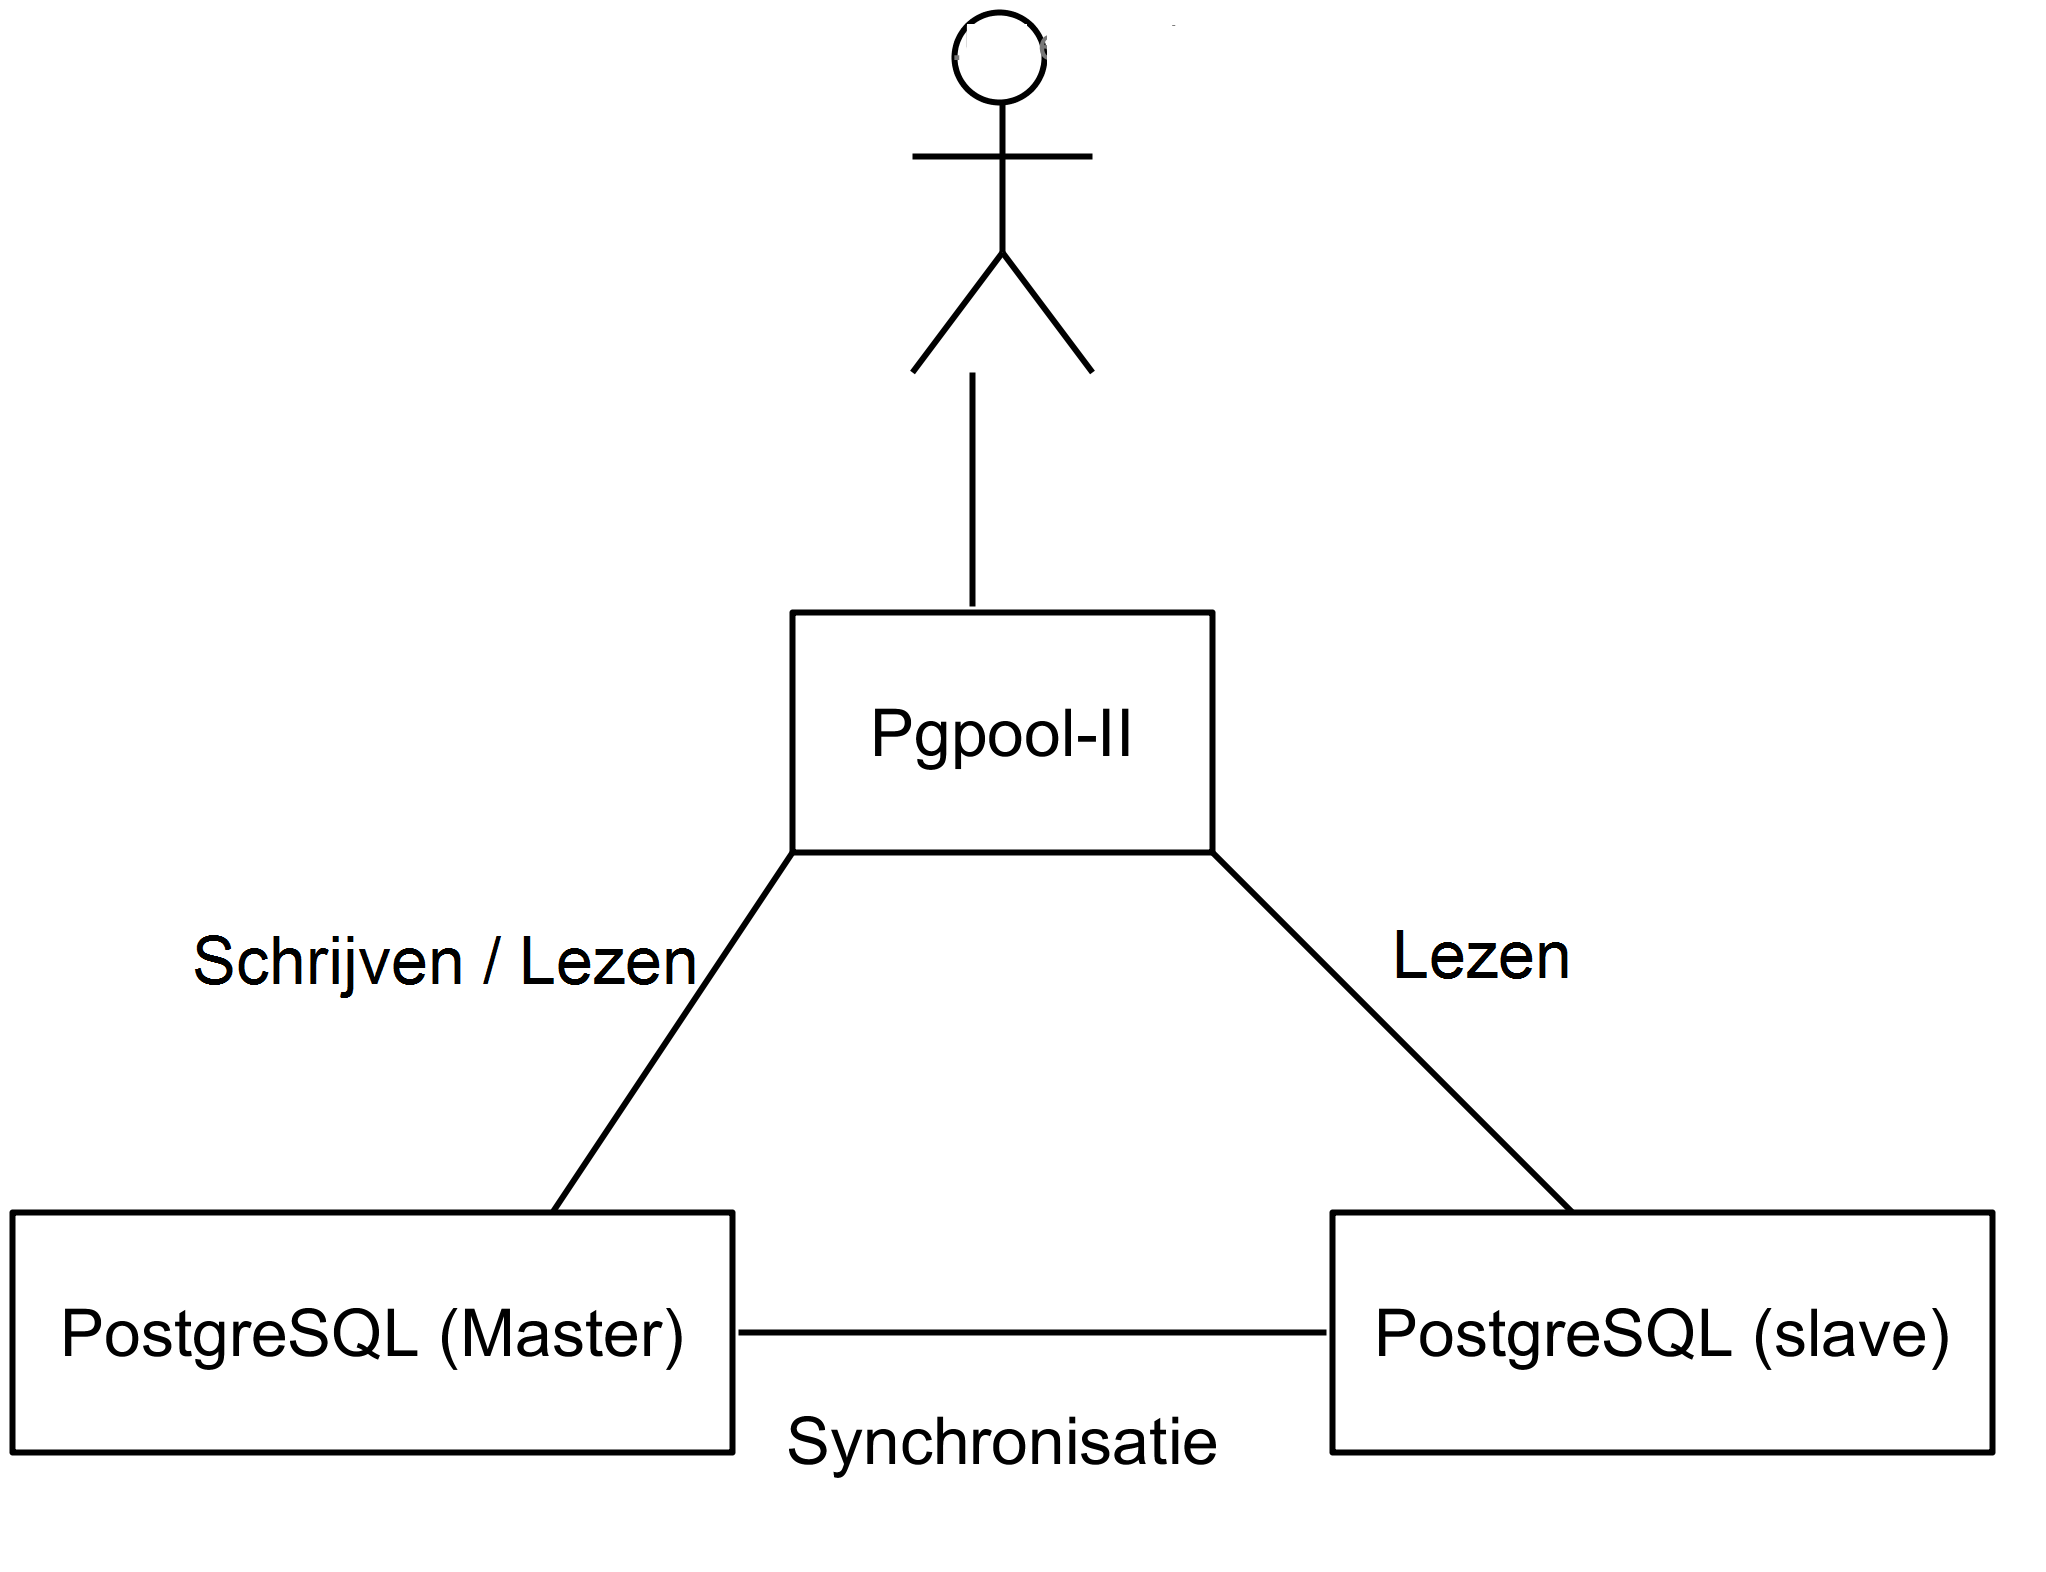
\includegraphics[width=0.5\linewidth]{img/Pgpool-structuur}
\caption{Systeemarchitectuur van Pgpool-II.}
\label{fig:Pgpool-structure}
\end{figure}

Op data niveau bestaat een individuele service uit een PostgreSQL installatie waarbij extra functies en bestanden worden geïnstalleerd met een aanpassing aan de configuratie bestanden.  Daarnaast moet er voor de online recovery ook ssh toegang voorzien worden tot al de PostgreSQL servers. De verschillende data machines hebben een master/slave structuur waar al de schrijfacties naar de master worden gestuurd en de leesoperaties zijn verdeeld over al de machines. De master doet aan synchronisatie met behulp van de \textit{Write-ahead-log} van PostgreSQL waar al de schrijfactie worden gelogd. 

Op routing niveau draait een Pgpool-II service die als management service dient, hij bepaalt wie master en slave is, volgt de status op van de data services en doet aan online recovery. Bij het aanmaken van een database connectie naar welke service de leesoperaties zullen gaan, zo wordt de leesbelasting verdeeld. 

Pgpool-II kan ook in de parallel mode werken zodat er de mogelijkheid is tot horizontale schaalbaarheid, ook is er de mogelijkheid om caching aan te zetten en een integratie met Memcache is ondersteund. 

\section{Selectie en uitwerking van de testsoftware}
De testen zijn geïmplementeerd als een uitbreiding van YCSB\cite{cooper2010benchmarking} omwille van verschillende redenen. Allereerst is de broncode publiek beschikbaar onder Apache 2.0, daarnaast is dit een uitgebreid systeem voor het uitvoeren van performantie benchmarking, dit op basis van het meten van de vertraging op een query voor verschillende DBMS's. Hierdoor heeft deze al een uitgebreide ondersteuning voor tal van DBMS's, waaronder al de gekozen systemen. Wel is deze ondersteuning nog verder geoptimaliseerd voor de gekozen systemen zodat er maximaal gebruik gemaakt wordt van de functionaliteiten van elk systeem. Een concreet voorbeeld, bij het opstellen van de scan queries rekening gehouden wordt met het aantal records dat nodig is wat standaard in YCSB niet gebeurd bij het uitvoeren op een relationele database. 

De 2 testen, beschikbaarheidstest en consistentie test, worden op verschillende manieren geïmplementeerd, naar de leidraad van sectie \ref{sec:testenvandesystemen}.  

\paragraph{Beschikbaarheidstest} De beschikbaarheidstest wordt geïmplementeerd door middel van \textit{event support}, hiermee kan er op vooraf gedefinieerde momenten een bepaald Unix commando uitgevoerd worden. De configuratie gebeurt met behulp van een XML bestand met de parameters van \ref{table:beschikbaarheidinput} in bijlage die meegegeven wordt aan de parameter $eventFile$, de output komt in het logbestand met de elementen van tabel \ref{table:beschikbaarheidoutput} in bijlage. 

Met behulp van deze uitbreiding zullen de beschikbaarheidstesten nadien uitgevoerd kunnen worden. Er zal gekeken worden naar de verandering in vertraging op een query waarmee kan bekeken worden of het systeem nog beschikbaar is. 

\paragraph{Consistentie testen} Voor de consistentie testen is er een extra module geïmplementeerd die het gedrag van sectie \ref{sec:testenvandesystemen} uitvoert. In deze uitwerking leest de schrijver niet zijn eigen data, al zou dit eenvoudig mee geïmplementeerd kunnen worden. Dit is niet getest omdat het niet nodig was in deze testen. De testen kunnen uitgebreid geconfigureerd worden om enkel te testen wat nodig is: een overzicht van de configuratie parameters, uitgezonderd de locatie van de logbestanden, is te vinden in tabel \ref{table:consistentieinput} in bijlage. Voor elke uitgevoerde query, wordt een record aangemaakt met de data van tabel \ref{table:consistentieuitvoer} in bijlage. 

De code van deze testen is beschikbaar op GitHub onder  \url{https://github.com/thuys/YCSB-Implementation}. 

\section{Installatie en opstelling van de DBMS's en YCSB}
Het uitvoeren van de testen vereist het opstellen van het volledige systeem en configuratie van de verschillende DBMS's. Voor het uitvoeren van de verschillende testen is het slechts nodig om het systeem een enkele keer op te zetten. Maar om de testen eenvoudiger te kunnen uitvoeren op verschillende infrastructuren en andere gebruikers de resultaten te laten controleren, is de installatie en configuratie van het systeem geautomatiseerd. 

De automatisatie gebeurt met het Integrated configuration Management Platform (IMP) beschreven in \cite{KULeuven-453199}. Dit modulair framework is uitgebreid met de 3 DBMS's en YCSB waardoor de configuratie als een declaratief gewenste staat wordt uitgedrukt. IMP zal deze staat toepassen op de verschillende systemen bij het uitrollen. 

Een uitgebreider bespreking van de uitwerking in IMP kan gevonden worden in bijlage \ref{chap:AppendixUitwerkingIMP} met het domeindiagram, uitleg en voorbeeldcode. 

Voor de uitvoering van de testen, is er voor elk DBMS gekozen voor een minimaal aantal instantie dat datadistributie én replicatie ondersteunt, voor de laatste eigenschap zou de data beschikbaar moeten zijn bij het uitvallen van 1 server. In de testen is er enkel gefocust op het uitvallen van dataservers, niet naar configuratieservers. Om deze reden zijn configuratieservers en minimaal opgezet. 

De opstelling van de systemen is getoond in figuur \ref{fig:deployment-testomgeving} in bijlage, elke uitrol van de systemen zal in meer detail besproken worden nadat de testinfrastructuur is besproken.  

De testinfrastructuur is een IaaS (Infrastructure as a Service) gebaseerd op OpenStack\footnote{https://www.openstack.org/}. De infrastructuur bestaat uit 3 Dell R610 en R620 servers met een totaal van 196GB RAM, 44 fysische CPU's (88 met hypertreading), verbonden met een Gigabit switch. Deze infrastructuur is gedeeld met andere gebruikers. Elke instantie heeft 2 virtuele CPU's, 4GB RAM en 50GB schijfruimte. De instanties worden verdeeld over de verschillende servers. 

\paragraph{HBase} Voor HBase wordt de data standaard 3 maal gerepliceerd en zijn er voor datadistributie dus 4 data instanties nodig die elk een HBaseRegionServer en Hadoop datanode zijn. Verder is er nog de nood aan een HMaster, Zookeeper en Hadoop namenode die samen op een enkele instantie worden uitgerold. In het totaal zijn er 5 instanties. Een overzicht van de infrastructuur getoond in figuur \ref{fig:HBase-deployment} in bijlage. De installatie en configuratiebestanden kunnen gevonden worden op \url{https://github.com/thuys/hbase}. 

\paragraph{Pgpool-II} Bij Pgpool-II is er ondersteuning voor horizontale schaalbaarheid in de parallel mode maar dit is niet getest. Om deze reden is er enkel replicatie toegepast waarvoor er 3 instanties zijn: een Pgpool-II instantie en twee PostgreSQL instanties. De configuratie van deze instanties zijn standaard met uitzondering van de activatie van de Write-Ahead-Log van PostgreSQL en de activatie van de replicatie mode in Pgpool-II. Een overzicht van de infrastructuur is getoond in figuur \ref{fig:pgpool-deployment} in bijlage. De installatie en configuratiebestanden kunnen gevonden worden op \url{https://github.com/thuys/postgresql}.

\paragraph{MongoDB} MongoDB heeft ondersteuning in replicatie en datadistributie. Voor het beschikbaar zijn van de data bij het uitzetten van een enkele instantie, zijn er 3 MongoDB datanodes nodig in een replicaset. De data wordt verdeeld over 2 replicaset met behulp van sharding op basis van de hash van de identificatie. Omdat de toegangsserver en configuratie instanties niet veel resources innemen, zijn deze verspreid over de verschillende data instanties, er zijn meerdere toegangsnodes geplaatst om bij de beschikbaarheidstesten steeds aan één node te kunnen. Zo zijn er in totaal 6 instanties nodig. Deze zijn beschreven in \ref{fig:MongoDB-deployment} in bijlage. De installatie en configuratiebestanden kunnen gevonden worden op \url{https://github.com/thuys/mongodb}.

\paragraph{YCSB} YCSB kan naar meerdere instanties uitgerold worden. Bij de calibratietesten zullen er 2 instanties gebruikt worden, maar er zal blijken dat dit niet een limiterende factor is. Voor het uitvoeren van de eigenlijke testen, zal er gebruik gemaakt worden van een enkele YCSB instantie, namelijk VM-1.  Een overzicht is getoond in figuur \ref{fig:YCSB-deployment} in bijlage. 


\section{Uitvoeren van de calibratie en testen}
Voor het uitvoeren van de volledige benchmarking dient eerst de verdeling van de type queries gespecificeerd worden, deze zijn voor alle verschillende systemen gelijk. Een overzicht van deze parameters kunnen gevonden worden in tabel \ref{table:calibratiequeries}. 40\% van de uitgevoerde queries past de database aan, er is dus een dynamische database. Bij het lezen wordt er de helft van de keren in batch gelezen met gemiddeld gezien 50 records per keer. Tenslotte wordt er met een \textit{zipfian} verdeling gekozen om regelmatig dezelfde records te lezen waardoor er uit cache gelezen worden. 

Voor later de data optimaal te kunnen analyseren, wordt er elke second de gemiddelde vertraging gelogd voor elk type query. 

\paragraph{Calibratie testen} Voor de calibratie van de omgeving zijn er 2 soorten testen gedraaid, de parameters voor het aantal connecties kunnen gevonden worden in tabel \ref{table:calibratiegebruikers}. De parameters voor het aantal queries per second zijn te vinden in tabel \ref{table:calibratiequeriesperseconde}, in dit geval is het aantal gebruikers afhankelijk van de vorige test. 

\begin{table}[htb!]
	\centering
	\begin{tabular}{l| l }
	\textbf{Naam} & \textbf{Waarde} \\
	\hline
	Aantal velden & 10 (1 key veld) \\
	Record grootte & 1KB (100byte/veld) \\
	Lees alle velden & true \\
	Invoeg queries (\textit{insert}) & 20\%\\
	Lees queries (\textit{select}) & 40\%\\
	Aanpas queries (\textit{update}) & 20\%\\
	Scan queries (\textit{scan}) & 20\%\\
	Opvraag verdeling & zipfian (\textit{bepaalde records worden} \\
	& \textit{veel gelezen, andere weinig}) \\
	Maximale scan grootte & 100 \\
	Verdeling scan grootte & uniform \\
	\end{tabular}
	\caption{Overzicht van de query parameters}
	\label{table:calibratiequeries}
\end{table}

\begin{table}[htb!]
	\centering
	\begin{tabular}{l| l}
	\textbf{Naam} & \textbf{Waarde}  \\
	\hline
	Ingeladen records  & 300 000 \\
	Pauze & 50s \\
	Executie tijd & 600s \\
	Aantal gebruikers & 1, 2, 3, 4, 5, 7, 10, 15, \\
	& 20, 30, 40, 50, 75, 100\\
	\end{tabular}
	\caption{Calibratie: Overzicht van de parameters voor het testen van het aantal gebruikers}
	\label{table:calibratiegebruikers}
\end{table}

\begin{table}[htb!]
	\centering
	\begin{tabular}{l| l  }
		\textbf{Naam} & \textbf{Waarde}  \\
		\hline
		Ingeladen records  & 300 000  \\
		Pauze & 50s  \\
		Executie tijd & 600s \\
		Theoretisch aantal records & 20, 50, 100, 150, 200, 250, 300, 400, 500, \\
		per seconde  & 600, 700, 800,  900, 1000, 2000, 2500, 3000\\
	\end{tabular}
	\caption{Calibratie: Overzicht van de parameters voor het testen van het aantal records per seconde}
	\label{table:calibratiequeriesperseconde}
\end{table}

\paragraph{Beschikbaarheidstesten} Bij het uitvoeren van de testen op beschikbaarheid van de verschillende systemen zijn de parameters in tabel \ref{table:beschikbaarheidstesten-parameters} gebruikt. Het aantal vooraf ingeladen records is op 300 000 geplaatst zodat zowel HBase als MongoDB aan sharding doen. De commando's voor het stoppen en starten van de systemen zijn te vinden in tabel \ref{table:beschikbaarheidstesten-commandos}.  Voor Pgpool-II is er een extra commando toegevoegd dat na het herstarten van de systemen wordt uitgevoerd, dit komt omdat er geen automatische recovery in Pgpool-II is. Tenslotte worden deze testen uitgevoerd op al de datanodes, een overzicht hiervan met de overeenkomstige service is te vinden in tabel \ref{table:beschikbaarheidstesten-nodes}. De testen voor MongoDB zijn enkel uitgevoerd op een enkele replicaset en dat is deze zonder enige configuratie servers. Een enkele replicaset is voldoende omdat de verschillende replicasets dezelfde functie hebben, enkel andere data opslaan. 

\begin{table}[ht!]
	\centering
	\begin{tabular}{l| l }
		\textbf{Naam} & \textbf{Waarde}  \\
		\hline
		Ingeladen records  & 300 000 \\
		Pauze & 50s \\
		Executie tijd & 900s \\
		Opstart kost & 100s \\
		Stoppen & Op 300s \\
		Starten & Op 600s \\
	\end{tabular}
	\caption{Beschikbaarheidstesten: Overzicht van de parameters}
	\label{table:beschikbaarheidstesten-parameters}
\end{table}


\begin{table}[ht!]
	\centering
	\begin{tabular}{l| l l }
		\textbf{Naam} & \textbf{Instanties} & \textbf{Service naam} \\
		\hline
		HBase  & HB2, HB3, HB4, HB5 & hbase-regionserver \\
		MongoDB  & MDB4, MDB5, MDB6, & mongodb-dataserver\\
		Pgpool-II  & PG1, PG2 & postgresql \\
	\end{tabular}
	\caption{Beschikbaarheidstesten: Overzicht van de instanties naar figuur \ref{fig:deployment-testomgeving}}
	\label{table:beschikbaarheidstesten-nodes}
\end{table}

\paragraph{Consistentie testen} Voor de consistentie testen moeten de parameters van tabel \ref{table:consistentieinput} geconfigureerd worden, de parameters zijn te vinden in tabel \ref{table:consistentie-testen-parameters}. Deze test wordt uitgevoerd op HBase en MongoDB. 

Om de analyse van de gegevens eenvoudiger te maken is er bij MongoDB gekozen om de test enkel uit te voeren op een replicaset en niet op een volledige cluster. Er is de aanname dat het consistentie venster bepaald is door de tijd dat het duurt dat de gegevens beschikbaar zijn op al de verschillende instanties van een replicaset, het testen van een cluster voegt zo extra complexiteit toe. Deze test zou in de toekomst ook uitgevoerd kunnen worden op een cluster maar is in dit geval niet gedaan.  

\begin{table}[htb!]
	\centering
		\begin{tabular}{l|c c }
			\textbf{Naam} & \multicolumn{2}{c}{\textbf{Waarde}} \\ 
		 	 & \textbf{HBase} & \textbf{MongoDB} \\ \hline
			Ingeladen records  & \multicolumn{2}{c}{300 000} \\
			Pauze & \multicolumn{2}{c}{50s} \\
			Executie tijd & \multicolumn{2}{c}{900s} \\	
			starttime & \multicolumn{2}{c}{30s} \\
			readThreads & 10 & 5\\ 
			consistencyDelayMillis & 30ms & 10ms\\ 
			newrequestperiodMillis & \multicolumn{2}{c}{500ms} \\ 
			readProportionConsistencyCheck & \multicolumn{2}{c}{50\%} \\ 
			updateProportionConsistencyCheck & \multicolumn{2}{c}{50\%} \\ 
			stopOnFirstConsistency & \multicolumn{2}{c}{True} \\ 
			maxDelayConsistencyBeforeDropInMicros & \multicolumn{2}{c}{300ms} \\ 
			timeoutConsistencyBeforeDropInMicro & \multicolumn{2}{c}{300ms} \\
		\end{tabular} 
	\captionof{table}{Consistentie testen: Overzicht van de parameters}
	\label{table:consistentie-testen-parameters}
\end{table}

\section{Verzamelen en analyse van de testresultaten}
De analyse van de data gebeurt aan de hand van de informatie die gelogd wordt tijdens de executie van de testen. Voor alle mogelijke testen maakt R-code de data visueel in verschillende grafieken. Voor elke test kan de data op een andere wijze voorgesteld worden. 

De uitleg en voorbeelden van deze grafieken zullen getoond worden bij het presenteren van de resultaten in het volgende hoofdstuk, op deze wijze is onmiddellijk een voorbeeld zichtbaar. 

De R code kan gevonden worden op GitHub \url{https://github.com/thuys/YCSB-R-Scripts}.  

\section{Conclusie}
In dit hoofdstuk is de vertaling gemaakt van een theoretisch testmodel tot de implementatie. Daarbij zijn keuzes gemaakt en bepaalde mogelijkheden zijn (nog) niet geïmplementeerd, dit is onder meer het geval voor lezen na het schrijven in de consistentie test, controleren of een waarde beschikbaar is in andere instanties na het platleggen van een instantie in de beschikbaarheidstest, ...

Maar de basis testmogelijkheden zijn geïmplementeerd en hiermee zijn al veel testen uit te voeren en conclusies te trekken op basis hiervan. In de volgende twee hoofdstukken zullen eerst de resultaten getoond worden en vervolgens een analyse van de resultaten op basis van de uitgevoerde testen.

